\documentclass[11pt]{article}
\usepackage[utf8]{inputenc}
\usepackage{amsmath}
\usepackage{amsfonts}
\usepackage{amssymb}
\usepackage{graphicx}
\usepackage[super]{nth}
\usepackage{amsthm}
\usepackage{bm}
\newtheorem{theorem}{Theorem}
\newtheorem{objective}{Objective}
\newtheorem{model}{Model}
\usepackage{xcolor}
\definecolor{light-gray}{gray}{0.95}
\newcommand{\code}[1]{\colorbox{light-gray}{\texttt{#1}}}
\usepackage{listings}
\usepackage{placeins}
\usepackage{enumitem}
\usepackage[T1]{fontenc}

\usepackage[authoryear]{natbib}

\lstset{language=R}


\makeatletter
\renewcommand{\maketitle}{
\begin{center}

\pagestyle{empty}

{\Large \bf \@title\par}
\vspace{1cm}

{\LARGE Marcel Gietzmann-Sanders}\\[1cm]

STAT651 - Statistical Theory I \\
University of Alaska Fairbanks


\end{center}
}\makeatother


\title{Homework 5}

\date{2025}
\setcounter{tocdepth}{2}
\begin{document}
\maketitle

\section*{Question 1}

\subsection*{a)}

The entire range over which $f_X(x)$ is non zero is positive, therefore we are taking a positive number to a real valued power which means $f_X(x)$ is non-negative. Therefore to confirm this is a pdf we need to ascertain whether its integral is exactly 1. Given $f_X(x)$ is not defined at zero we'll need to be careful about this.

$$\lim_{\epsilon^+ \rightarrow 0} \int_{\epsilon}^4 0.25x^{-1/2}dx=\lim_{\epsilon^+ \rightarrow 0} \left( 0.5 \sqrt{x} \Big|_{\epsilon}^{4} \right)=\lim_{\epsilon^+ \rightarrow 0} \left( 1 - 0.5 \sqrt{\epsilon} \right) = 1$$

This is indeed a pdf. 

\begin{figure}[h!] 
	\centering
  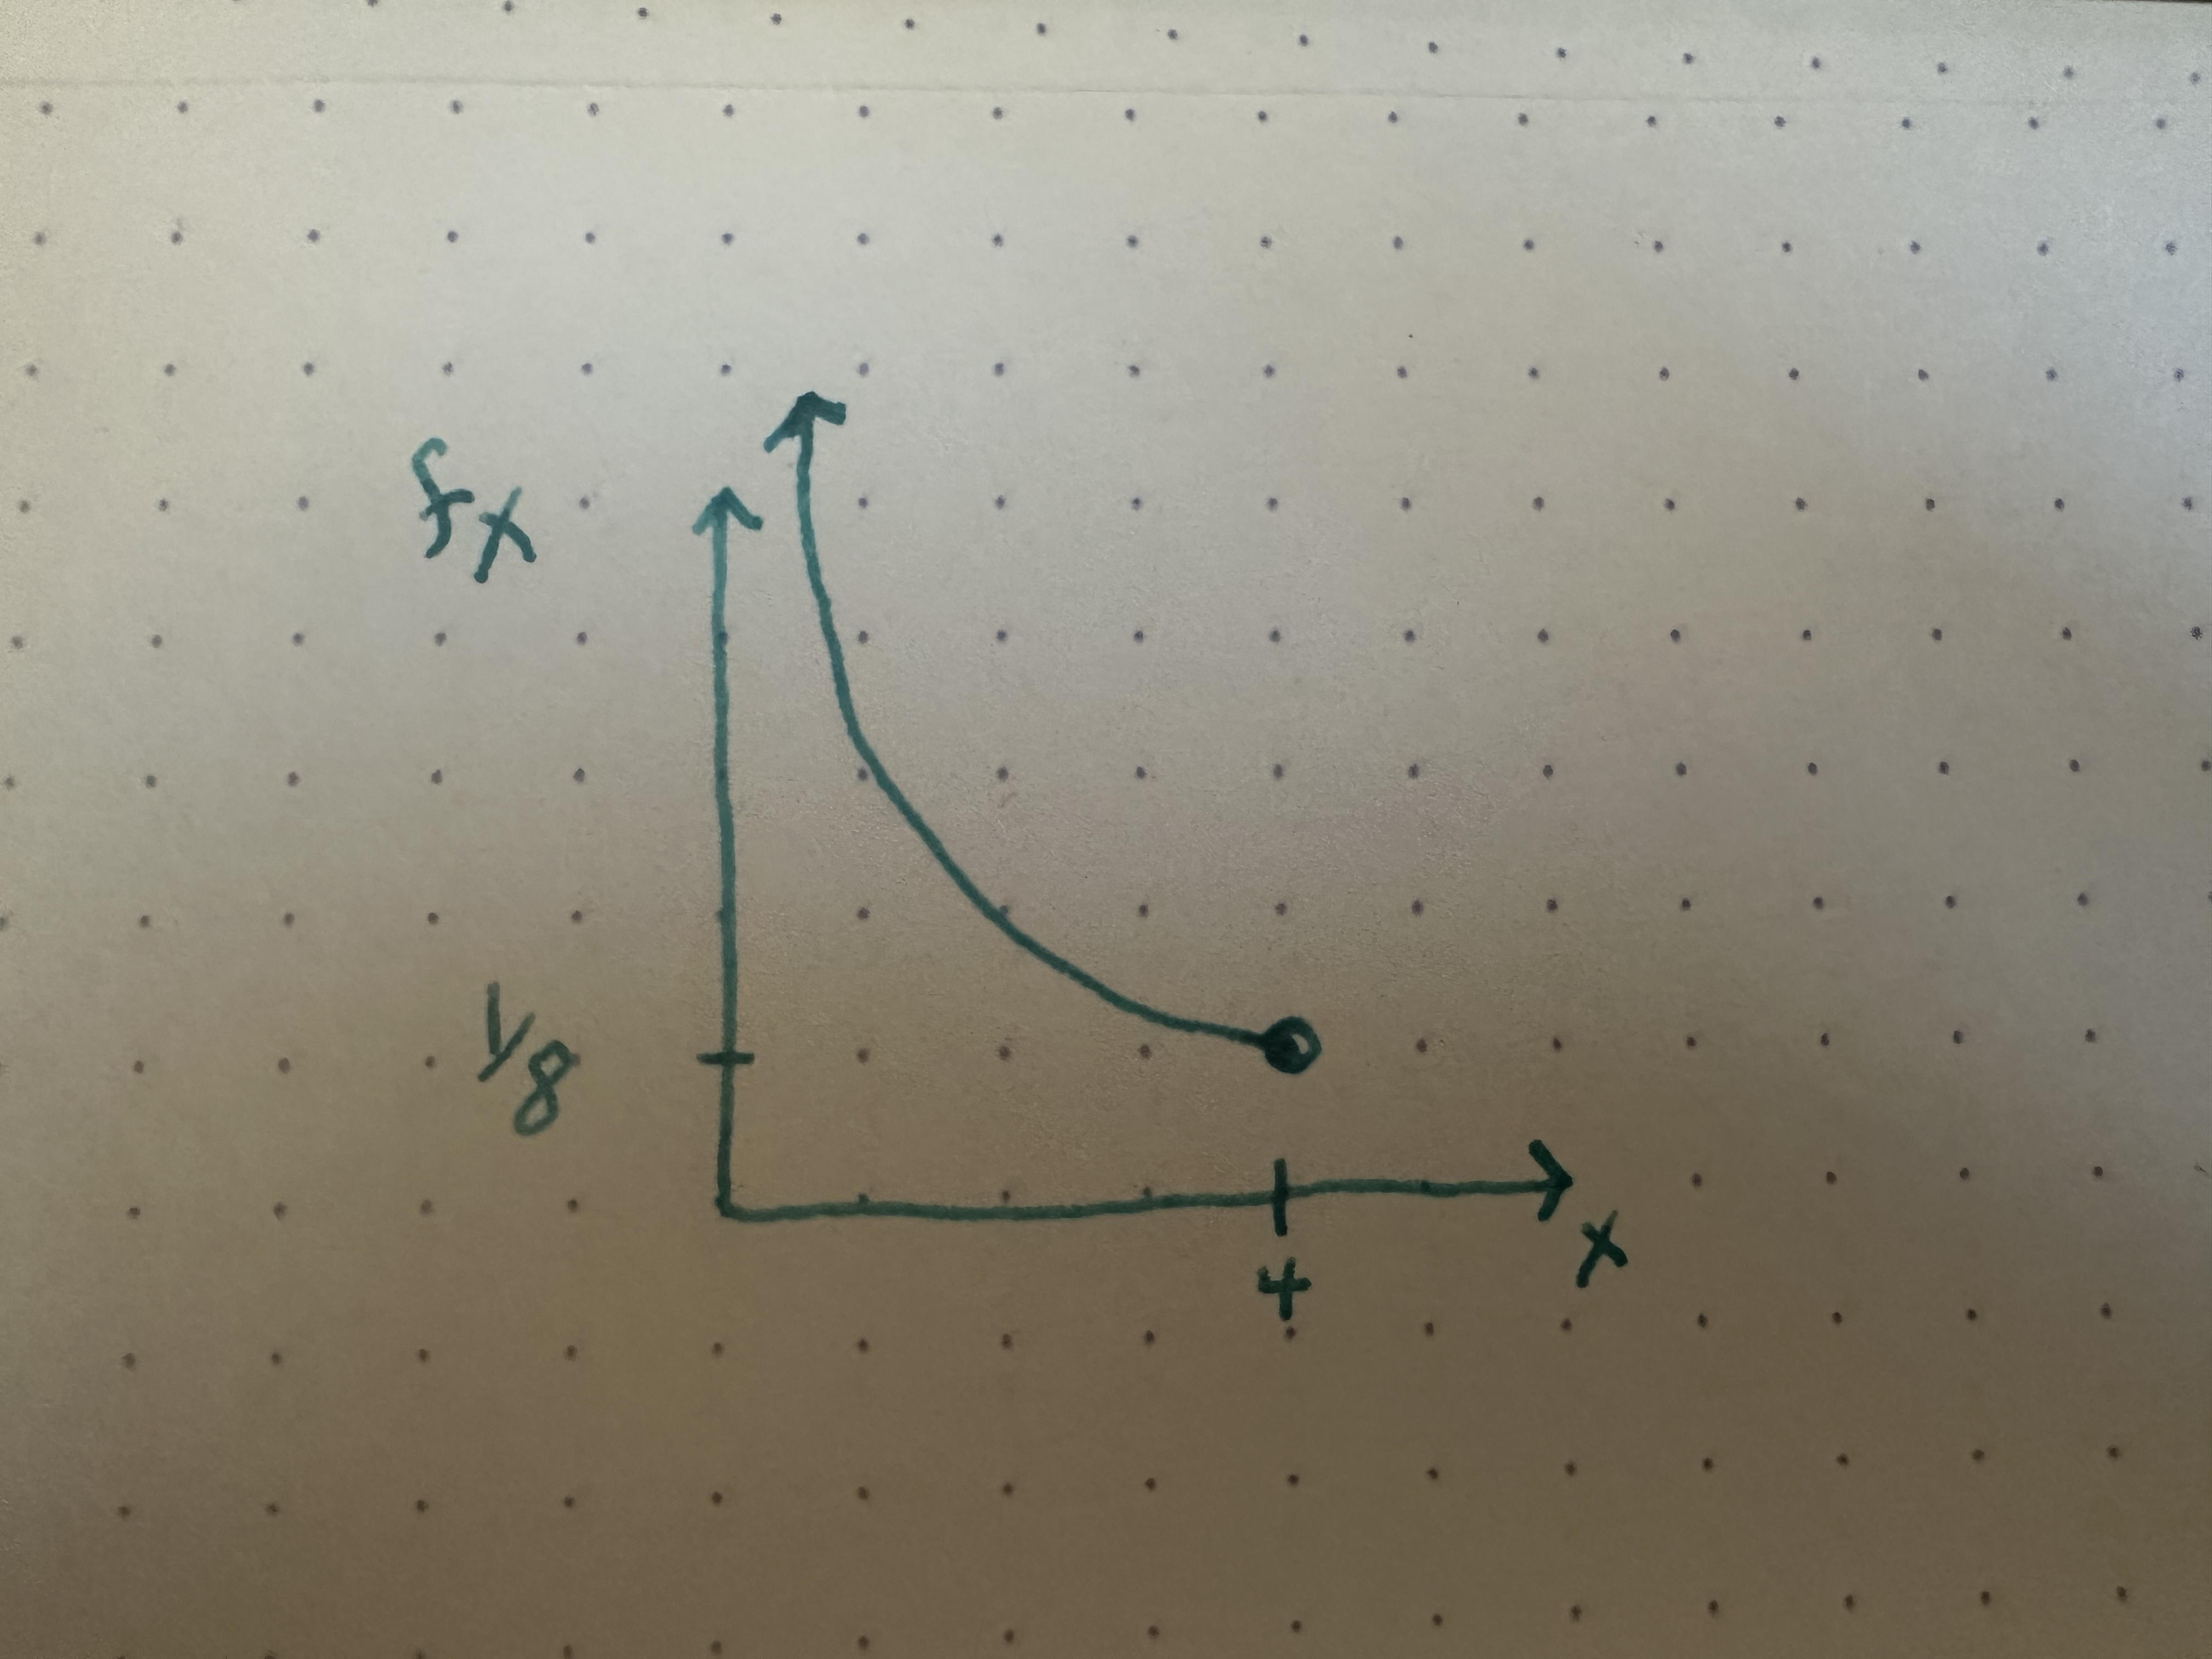
\includegraphics[height=60mm]{HW5Q1a.png}
  \label{fig:tree}
\end{figure}

\FloatBarrier

\subsection*{b)}

$$\mathbb{E}(X^3)=\lim_{\epsilon^+ \rightarrow 0} \int_{\epsilon}^4 x^30.25x^{-1/2}dx=0.25\int_{0}^4 x^{5/2}dx$$
$$=0.25\left( \frac{2}{7} x^{7/2} \Big|_0^4 \right)\approx 9.14$$

\subsection*{c)}

$g(x)=x^3$ which over the range of $(0, 4)$ is a monotonic function. $g(x)$ is also invertible over this range. Therefore:

$$f_Y(y)=f_X(g^{-1}(y))\Big| \frac{dx}{dy} \Big| = \left( 0.25 (y^{1/3})^{-1/2} \right)\frac{1}{3}y^{-2/3}=\frac{1}{12}y^{-5/6}$$

$$\mathbb{E}(Y) = \lim_{\epsilon^+ \rightarrow 0} \int_{\epsilon}^{64} y \frac{1}{12}y^{-5/6}dy=\frac{1}{12}\int_0^{64}y^{1/6}dy =\frac{1}{12}\left(\frac{6}{7}y^{7/6} \Big|_0^{64} \right) \approx 9.14$$

\section*{Question 2}

\subsection*{a)}

Let $A_1=(-1, 0)$ and $A_2=[0, 1)$ ($A_0=\emptyset$). Let $g_1(x) = 1 + x$ and $g_2(x) = 1 - x^2$. Both of these are monotone over their respective sets $A_1$ and $A_2$. Their range is also the same - $(0, 1]$. And the inverses $g_1^{-1}(y)=y-1$ and $g_2^{-1}(y)=\sqrt{1-y}$ have derivatives $1$ and $-1/(2\sqrt{1-y})$ which are continuous over the range $(0, 1]$. Therefore we can apply Theorem 2.1.8 which says that:

$$f_Y(y)=\sum_{i=1}^2 f_X\left(g_i^{-1}(y)\right)\Big| \frac{d}{dy}g_i^{-1}(y) \Big|$$

$$=\left[ \frac{3}{8}(y-1+1)^2(1)\right]+\left[ \frac{3}{8}(\sqrt{1-y}+1)^2\left( 1/(2\sqrt{1-y})\right) \right]$$

$$=\frac{3}{8}\left[ y^2 +\frac{1-y+2\sqrt{1-y}+1}{2\sqrt{1-y}}\right]$$

$$=\frac{3}{8}\left[ y^2 + 1 +\frac{1}{2}\left(\sqrt{1-y}+\frac{1}{\sqrt{1-y}}\right)\right]$$

\subsection*{b)}

We already know it's positive so all we need to do is show it integrates to 1. 

$$\lim_{\epsilon^- \rightarrow 1} \int_{0}^{\epsilon} \frac{3}{8}\left[ y^2 + 1 +\frac{1}{2}\left(\sqrt{1-y}+\frac{1}{\sqrt{1-y}}\right)\right] dy$$
$$=\lim_{\epsilon^- \rightarrow 1}\frac{3}{8}\left[1/3y^3 + y - 1/3(1-y)^{3/2} - \sqrt{1-y} \right] \Big|_{0}^{\epsilon}$$
$$=\frac{3}{8} \left[1/3 + 1 + 1/3 + 1 \right]=1$$

Therefore this is indeed a pdf!

\section*{Question 3}

From Theorem 2.1.10 we know $Y=F_X(x)$ will give us what we want. Therefore we just need to find the cdf of $X$. On the range $x\in(-2, 3)$ we have:

$$F_X(x)=\int_{-2}^{x} \frac{2}{25}(t+2)dt=\frac{2}{25}\left(\frac{1}{2}t^2+2t\right)\Big|_{-2}^{x}=\frac{2}{25}(0.5x^2 + 2x) + \frac{4}{25}$$
$$=\frac{2}{25}(\frac{1}{\sqrt{2}}x+\sqrt{2})^2$$

Therefore:

\[
Y = u(X) = F_X(X) = 
\begin{cases}
    0 & X \leq -2 \\
    \frac{2}{25}(\frac{1}{\sqrt{2}}X+\sqrt{2})^2 & X \in (-2, 3) \\
    1 & X \geq 3
\end{cases}
\]

So now:

$$F_Y(y) = P\left(X > \sqrt{25y}-2\right)$$ 

which as $y$ only ranges from $0$ to $1$ means:

$$F_Y(y) = P\left(X > \sqrt{25y}-2\right)=\frac{2}{25}(\frac{1}{\sqrt{2}}(\sqrt{25y}-2)+\sqrt{2})^2=y$$

which is precisely the cdf of a uniform distribution over $[0, 1]$.  

\section*{Question 4}

$$x_{n+1} = (2x_n + 5) \mod 16$$

\subsection*{a)}

1, 7, 3, 11, 11, 11,... 

\subsection*{b)}

4, 13, 15, 3, 11, 11,... 

\subsection*{c)}

11, 11, 11,...

\section*{Question 5}

\subsection*{a)}

$$\mathbb{E}(X) = \sum_x xf(x) = (1)0.3+(2)0.1+4(0.6) = 2.9$$

\subsection*{b)}

$$\frac{d}{dt}M_X(t)=0.3e^t+0.2e^{2t}+2.4e^{4t}$$

\subsection*{c)}

$$\frac{d}{dt}M_X(0)=0.3+0.2+0.24=2.9$$

\section*{Question 6}

The median occurs where the cumulative probability is 0.5.

\subsection*{a)}

$$F_X(x) = \int_0^x 5t^4dt=t^5 \Big|_0^x = x^5$$

Therefore our median is where:

$$x^5=0.5 \rightarrow x=(0.5)^{1/5}\approx 0.871$$

\begin{figure}[h!] 
	\centering
  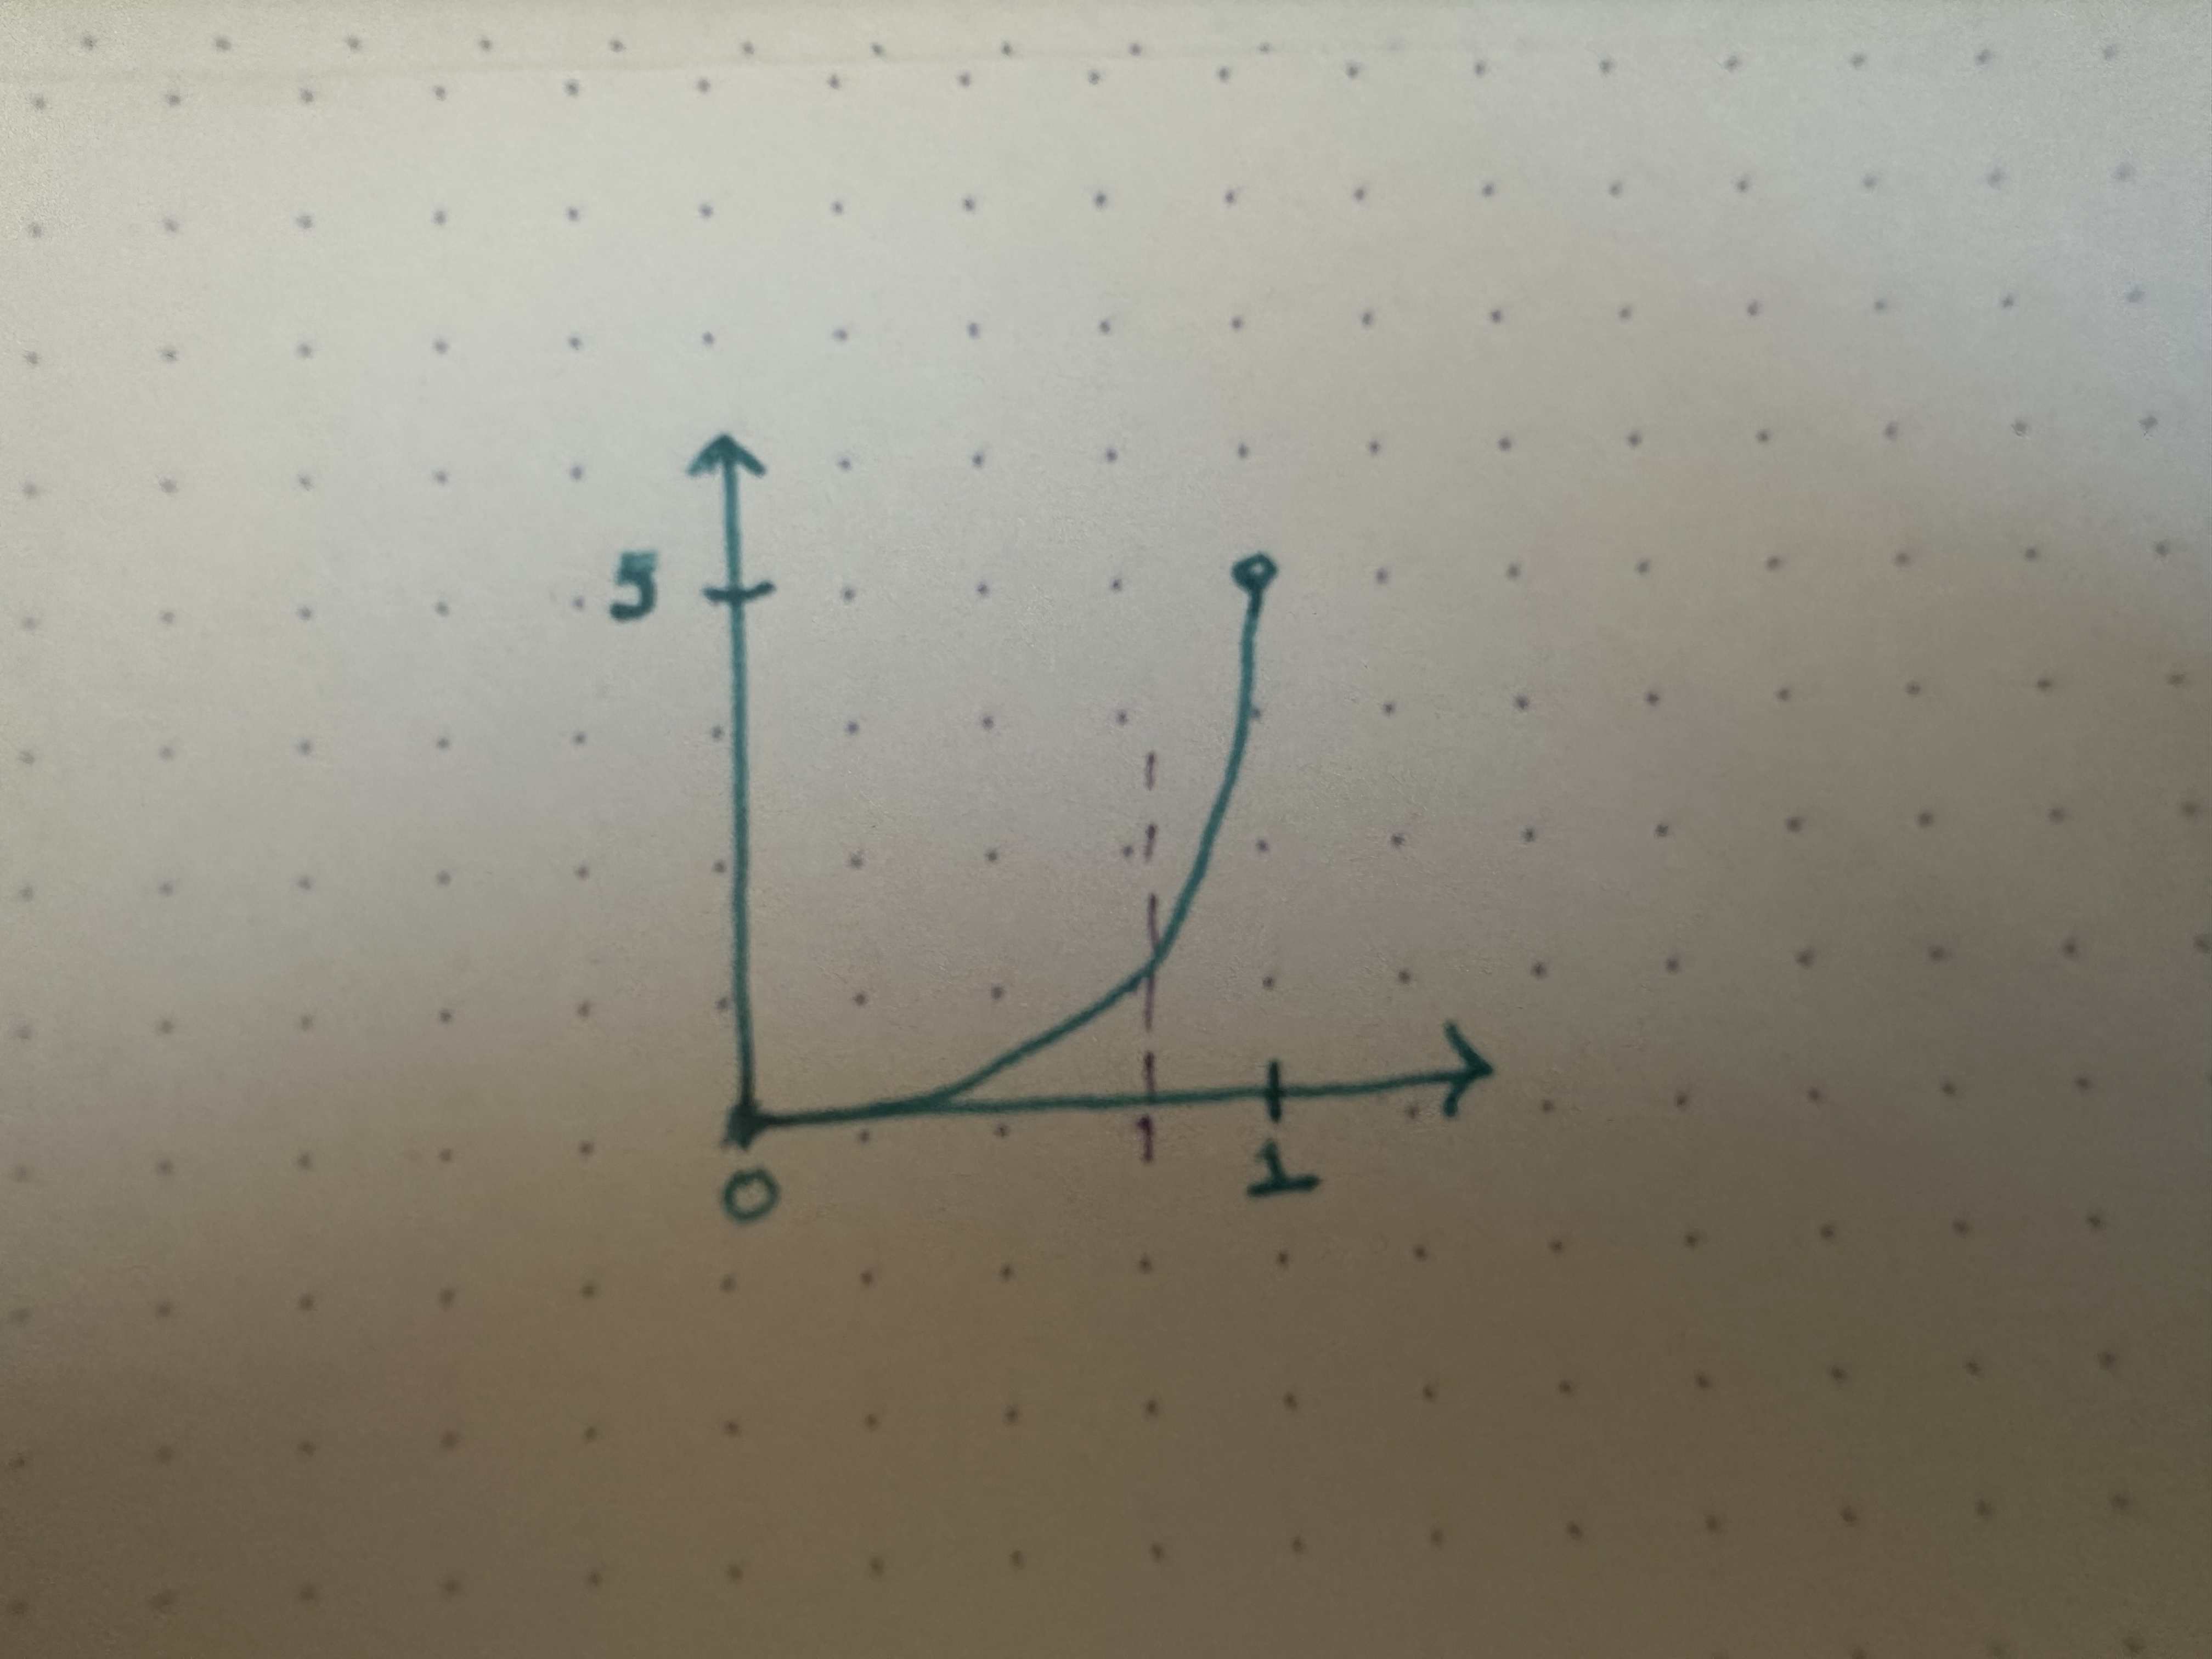
\includegraphics[height=60mm]{HW5Q6a.png}
  \label{fig:tree}
\end{figure}

\FloatBarrier

\subsection*{b)}

$$F_X(x) = \int_3^x 7e^{-7(t-3)}dt=-e^{-7(t-3)}\Big|_3^x=1-e^{-7(x-3)}$$

Therefore our median is where:

$$1-e^{-7(x-3)}=0.5 \rightarrow x=-\ln(0.5)/7+3\approx 3.1$$

\begin{figure}[h!] 
	\centering
  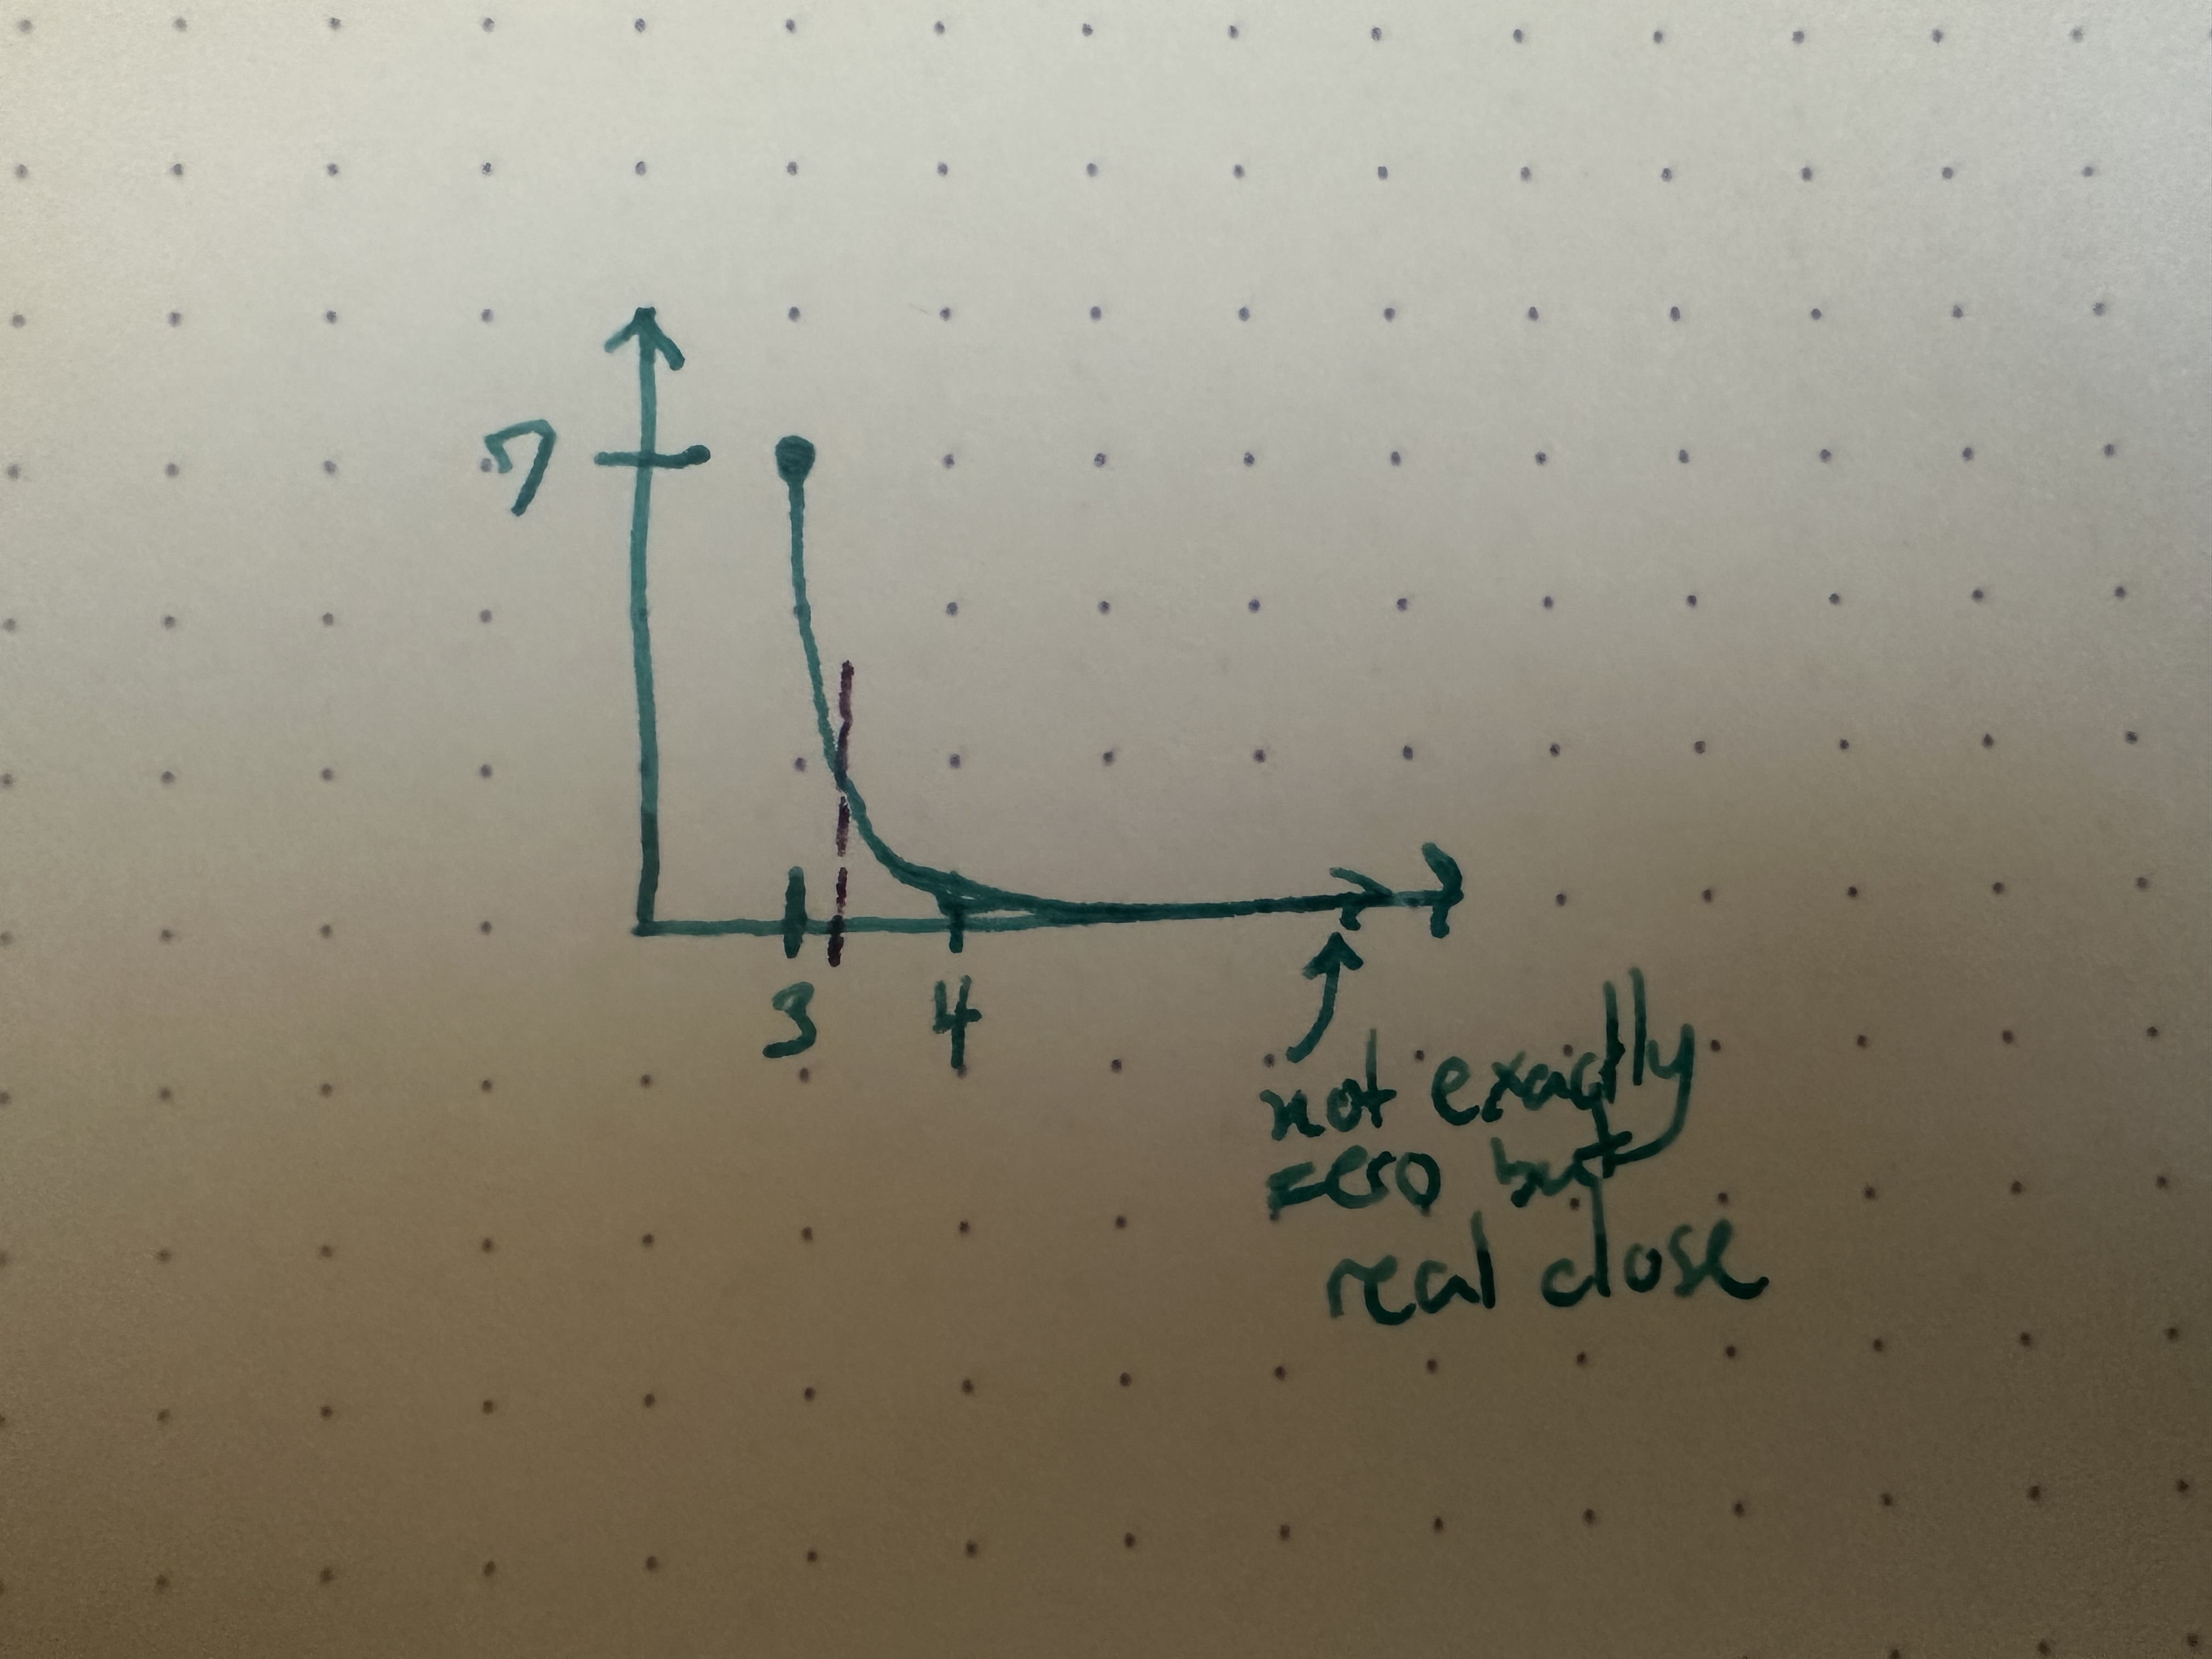
\includegraphics[height=60mm]{HW5Q6b.png}
  \label{fig:tree}
\end{figure}

\FloatBarrier

\section*{Question 7}

Let's call the calves thing one and thing two. Let $F_1$ be the set of events where thing one is a female and $F_2$ be the set of events where thing two is a female. So me knowing one of them is a female means either $F_1$ or $F_2$. This probability is:

$P(F_1 \cup F_2) = P(F_1) + P(F_2) - P(F_1 \cap F_2)=1/2 + 1/2 - 1/4=3/4$

This makes sense as the only event not in this union is if both thing one and thing two are male (1/4 of the options). 

So now I want to know - $P(F_1 \cap F_2 | F_1 \cup F_2)$ - that is, what is the probability they are both female given I know at least one of them is. 

$$P(F_1 \cap F_2 | F_1 \cup F_2) = P(F_1 \cap F_2) / P(F_1 \cup F_2) = 1/4(4/3) = 1/3$$

\end{document}